\section*{Conclusions}

The first important conclusion that come to mind is the fact that a problem that has no solution can be verified. Complexity theory has taught us that there can be a large gap between the complexity of verification versus search, but it has always been a difference of efficiency: if solutions to a problem can be verified then solutions can also be found (even if with drastically higher computational cost). This result show us that, with quantum entanglement, there can be a chasm of computability between verifying solutions and finding them.


There are still many things that are not clear. First of all: what is the role of entanglement here. What we have shown goes in the opposite direction of what the result seems to be. Entanglement makes the provers even more powerful, but in the end seems to make the verifier more efficient.
\begin{itemize}

    \item Construct an explicit $II_1$ factor that doesn't satisfy Connes'embedding property
    \item We could consider the complexity class $\text{MIP}^\text{co}$, which stands for \emph{multiprover interactive proofs in the commuting-operator model}. As always, we consider only two-prover one-round protocols. We know that this is contained in co-RE, namely the complement of RE. One could ask if $\text{MIP}^\text{co}$ = co-RE sussist.
    
\end{itemize}

An important conclusion is that it seems like quantum computer are inherently more powerful in verifying problem rather than solving problem. Let us explain.

At the moment we have the following situation

\begin{figure}[htb]
    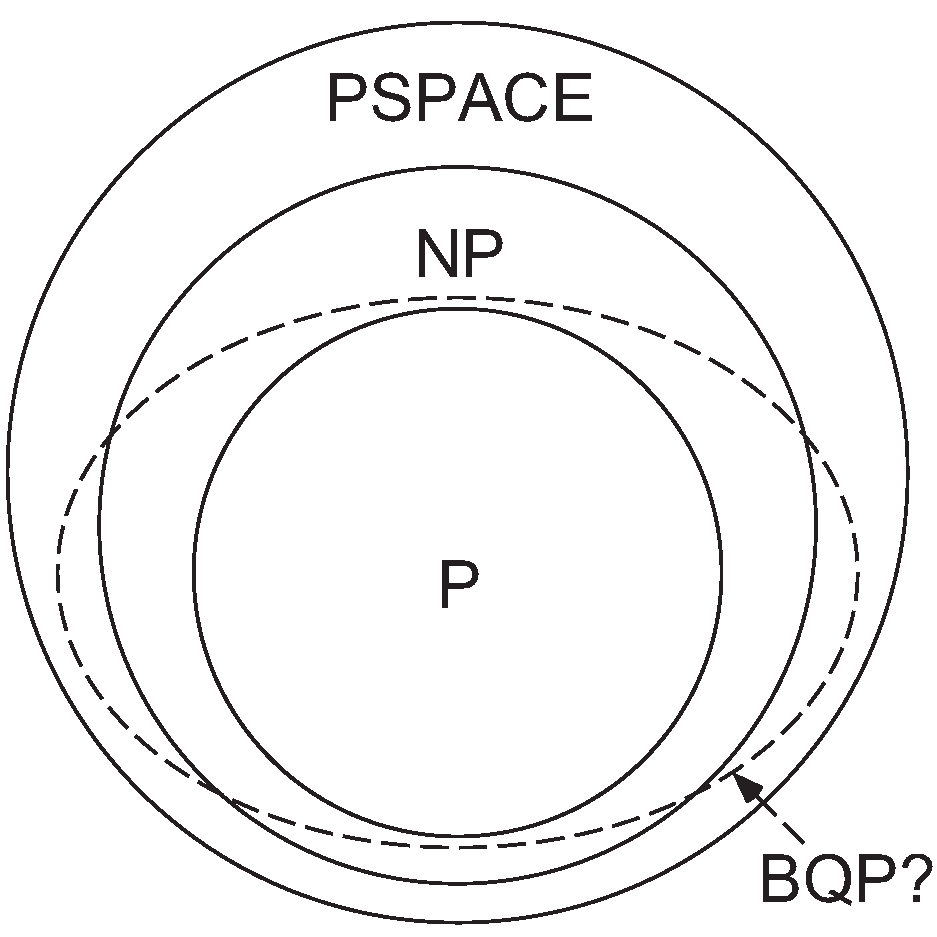
\includegraphics[width=\linewidth]{Quantum-complexity.png}
    \centering
    \caption{Complexity classes hierarchy.}
    \end{figure}